\chapter{Instalacja i wdrożenie}
\thispagestyle{chapterBeginStyle}

\textbf{UWAGA:} Poniższy opis przedstawia sposób instalacji odpowiednich pakietów dla komputerów korzystających z systemu operacyjnego 
\textbf{Linux}, a dokładniej- dystrybucji \textbf{Ubuntu}. Użytkownik chcąc zainstalować aplikację wraz z jej komponentami na 
komputerze z innym systemem operacjnym zobowiązany jest do samodzielnego zapoznania się ze wszystkimi komendami bądź mechanizami 
umożliwającymi instalację wskazanych pakietów.

\section{Instalacja pakietu SWI-Prolog}
\label{SWI-PROLOGRozdzial}
    Korzystając z dystrybucji Linuxa o nazwie Ubuntu, wystarczającą czynnością do poprawnej instalacji pakietu SWI-Prolog jest uruchomienie 
    następującej komendy z poziomu linii komend \texttt{sudo apt install swi-prolog-core}.
    
    Należy pamiętać o wymogu posiadania praw adminsitratora na komputerze, na którym dokonywany jest proces instalacji.
    W momencie, w którym komputer zakończy pobieranie oraz instalację pakietu wprowadzenie komendy \textit{swipl} powinno spodoować uruchomienie 
    interaktywnego interpretera języka PROLOG. Jeśli powyższa czynność zakończyła się sukcesem, komputer jest gotowy do uruchomienia kodu źródłowego 
    algorytmu oraz rozpoczęcia pracy nad kreowanie odpowiednich planów
\section{Instalacja języka Python}
    \label{InstallPython}
    Większość dystrybucji Linuxa posiada wbudowany w sobie język programowania python. Z reguły można to zweryfikować poprzez wpisanie komendy 
    \texttt{python3 --version}
    Należy zauważyć, iż wszystkie komponenty zostały napisane dla wersji języka python 3.x. Użytkownik korzystając ze starszych wersji 
    może spotkać się z anomaliami negatywnie wpływającymi na funkcjonowanie aplikacji, dlatego zaleca się korzystanie ze wskazanej powyżej wersji. \\
    Do poprawnego uruchomienia aplikacji wymagane są następujaće biblioteki 
    \begin{itemize}
        \item Tkinter
        \item graphviz 
        \item PIL
        \item pyswip
    \end{itemize}
    Poniżej znajdują się odpowiednie komendy, których użycie z poziomu linii komend zagwarantuje poprawne uruchomienie aplikacji:
    \begin{listing}[H]
        \begin{verbatim}
            sudo apt install python3-tk
            pip3 install graphviz
            pip3 install Pillow
            pip3 install pyswip
        \end{verbatim}
        \caption{Instalacja odpowiednich bibliotek dla języka python}
    \end{listing}
    Przed uruchomienie powyższych komend użytkownik winien posiadać zainstalowany pakiet \textit{pip}. Jeśli pobieranie wskazanych bibliotek zakończy 
    się błędem, należy uprzednio wykonać następującą komendę: \texttt{sudo apt install python3-pip} .
    Całą aplikację również jest uruchamiana z poziomu linii komend. Po pobraniu odpowiednich plików, w folderze \texttt{sources} znajduje się plik
    \texttt{gui.py}, który zawiera kod rozruchowy interfejsu użytkownika. \\
    Będąc we wskazanym katalogu należy uruchomić terminal i wprowadzić następującą
    komendę: \texttt{python3 gui.py}
    Jeśli operacja zakończy się sukcesem, użytkownik powinien ujrzeć okienko identyczne do tego, które zostało przedstawione w ramach sekcji \ref{GUIRozdzial}

\section{Dokumentacja}
    W katalogu \texttt{sources} (patrz Dodatek~\ref{plytaCD}) znajduje się katalog \texttt{html}. W nim, przy pomocy popularnego narzędzia \textbf{Doxygen},
    który jest automatycznym generatorem dokumentacji dla wielu popularnych języków programowania (w tym także dla pythona), wygenerowano plik \\
    o nazwie 
    \texttt{index.html}. Naciśnięcie na ów plik dwukrotnie przy pomocy lewego przycisku myszy powinno uruchomić przeglądarkę, w której, w formie strony
    internetowej, zostanie użytkownikowi przedstawiona pełna dokumentacja zaimplementowanych mechanizmów. \\

    \begin{figure}[H]
        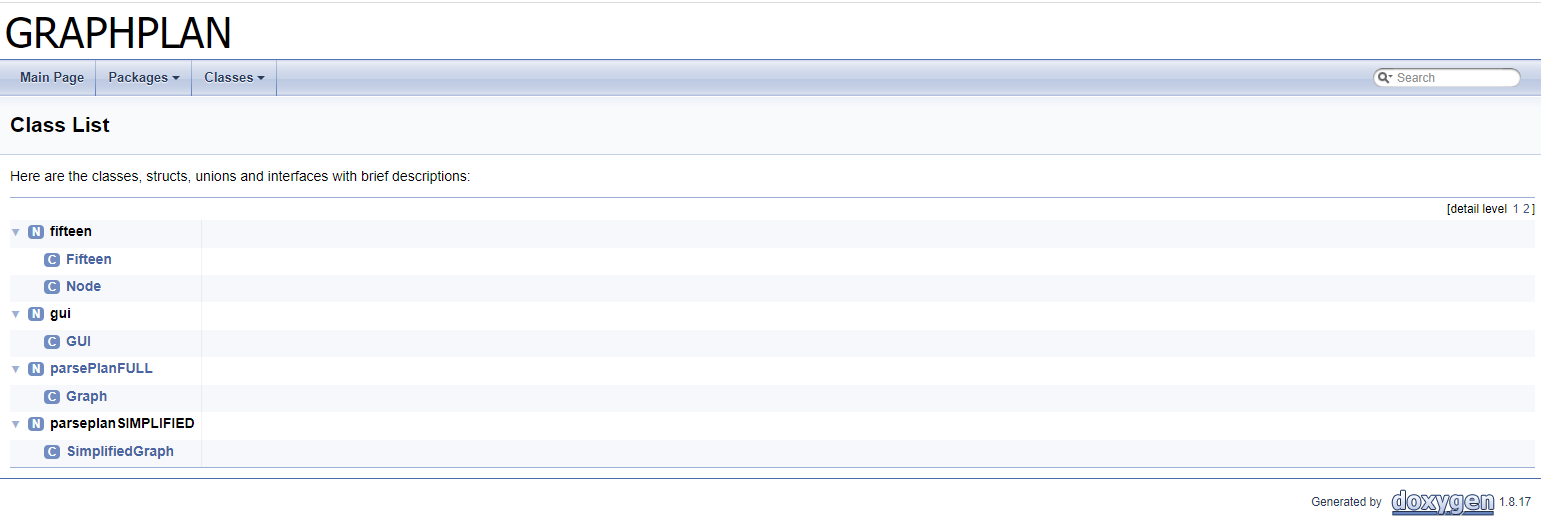
\includegraphics[scale=0.4]{SpisKlas}
        \centering
        \caption{Spis udostępnionych klas}
    \end{figure}

    \begin{figure}[H]
        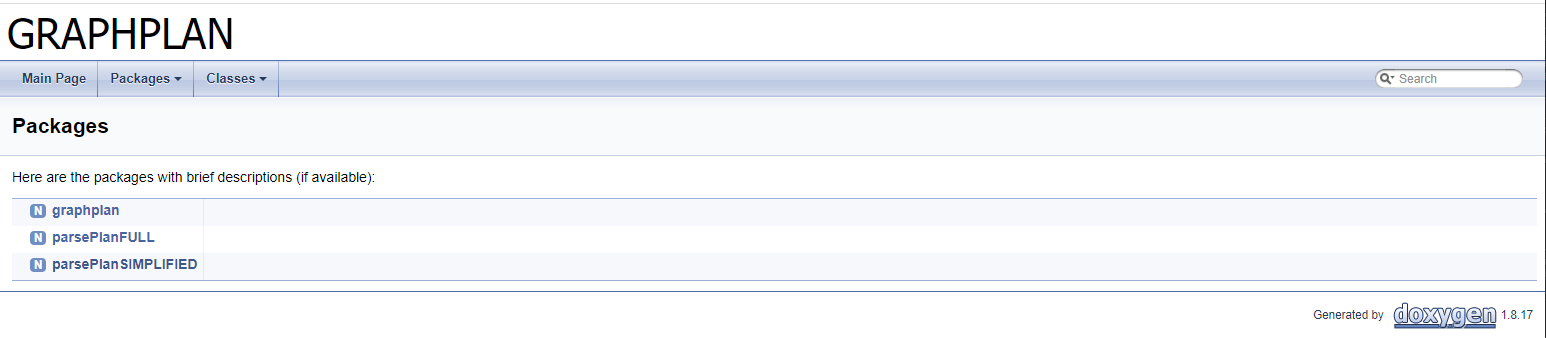
\includegraphics[scale=0.4]{SpisPaczek}
        \centering
        \caption{Spis udostępnionych paczek}
    \end{figure}

    \begin{figure}[H]
        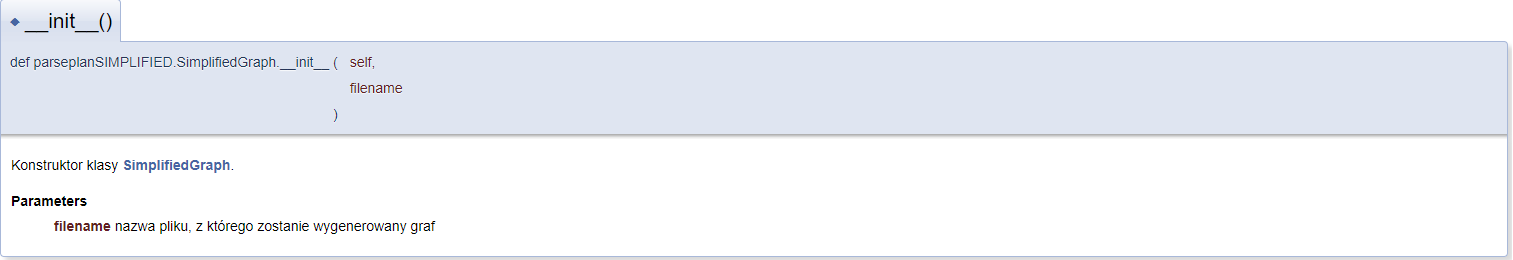
\includegraphics[scale=0.4]{OpisFunkcji}
        \centering
        \caption{Przykład opisu zaimplementowanej funkcji}
    \end{figure}
